\section{Time and Frequency Synchronization}
\subsection{The Problem of Synchronization}
\begin{figure}[H]
	\centering
	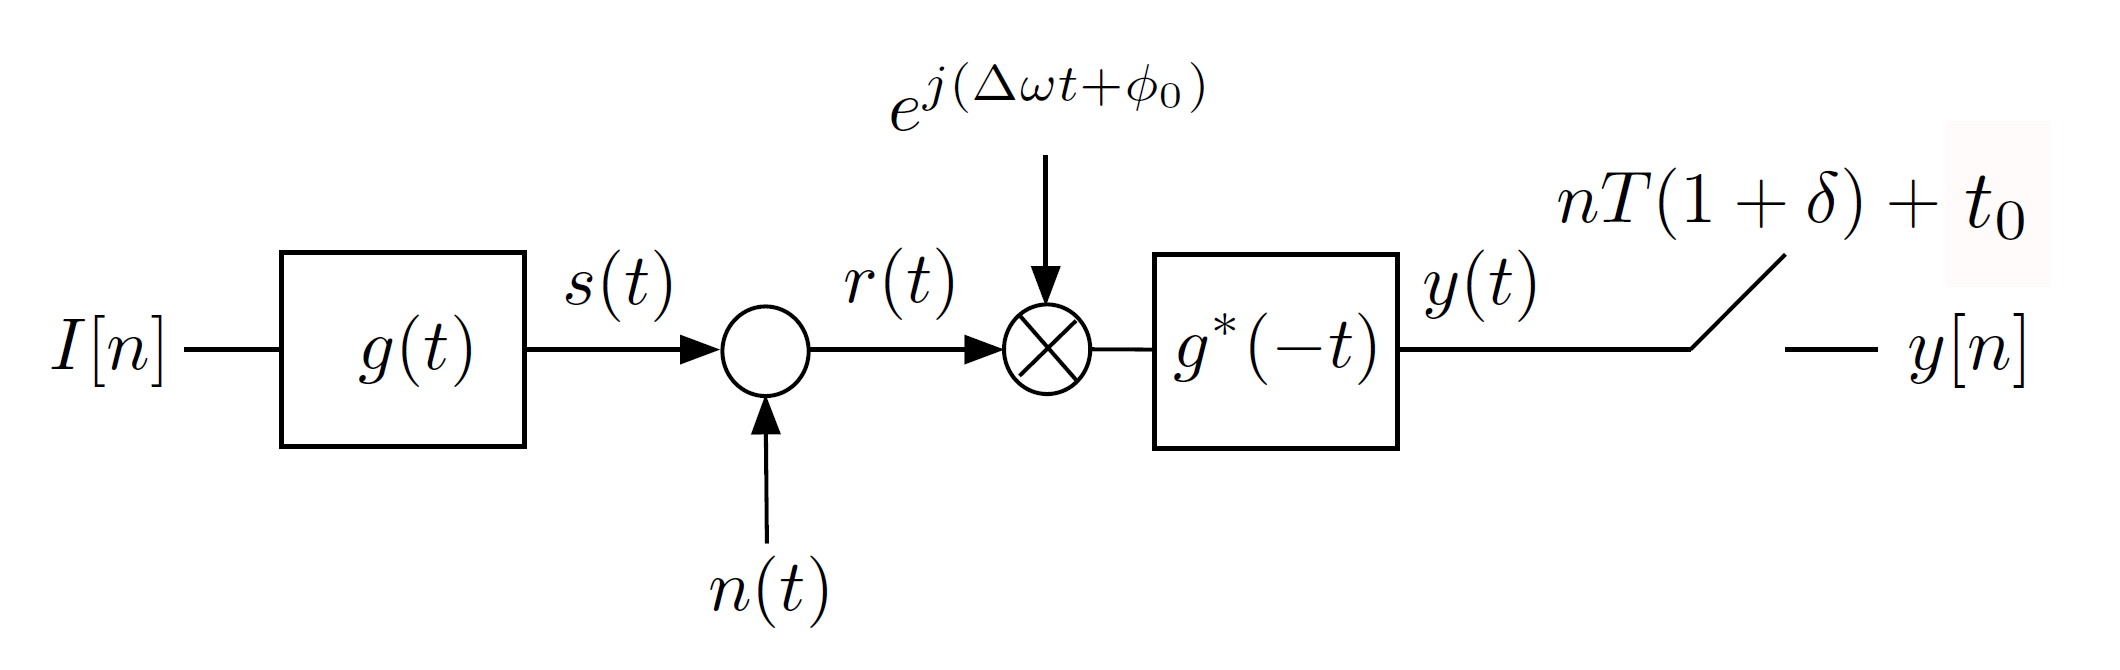
\includegraphics[width=\linewidth]{sync-errors-conceptual} % Path: Images/sync-errors-conceptual
	\caption{Synchronization mismatches at the receiver}
	\label{fig:sync-errors-conceptual}
\end{figure}
Accurate demodulation requires the transmitter and receiver to be synchronized. The receiver must precisely determine symbol sampling instances and align its local carrier frequency and phase with the received signal. Synchronization errors primarily arise because transmitter and receiver operate with independent local oscillators, which can have slight frequency deviations due to manufacturing imperfections or environmental factors. Additionally, signal propagation delay introduces an unknown carrier phase shift and symbol timing offset.\par
These phenomena lead to four main types of synchronization errors:
\begin{itemize}
	\item Carrier Frequency Offset (CFO), $\Delta f$: The difference between the transmitter's and receiver's carrier frequencies.
	\item Carrier Phase Offset, $\phi_0$: The phase difference between the incoming carrier and the receiver's local oscillator.
	\item Sample Clock Offset (SCO), $\delta$: The frequency mismatch between the transmitter's DAC clock and the receiver's ADC clock. This error was considered negligible and not implemented in this project.
	\item Sample Time Shift, $t_0$: The receiver's uncertainty about the exact arrival time of symbols, necessitating determination of optimal sampling instants.
\end{itemize}
Figure \ref{fig:sync-errors-conceptual} conceptually illustrates these mismatches, where transmitter symbols generated at $nT_{symb}$ are effectively sampled at $nT_{symb}(1+\delta)+t_0$ by the receiver.


\subsection{Impact of Synchronization Errors on Performance}
\subsubsection{Impact of Carrier Phase Offset ($\phi_0$)}
A static carrier phase offset, $\phi_0$, resulting from the phase difference between the incoming carrier and the receiver's local oscillator, causes a rotation of the entire received symbol constellation by an angle $\phi_0$ in the complex plane. Assuming perfect timing, no CFO, and no noise, a transmitted complex baseband symbol $I[n]$ becomes at the matched filter output:
\begin{equation}
	y[n] = I[n]e^{j\phi_0}
\end{equation}
\par
This rotation, if uncorrected, leads to incorrect decisions at the detector.

\subsubsection{Impact of Carrier Frequency Offset ($\Delta f$)}
\begin{figure}[H]
    \centering
    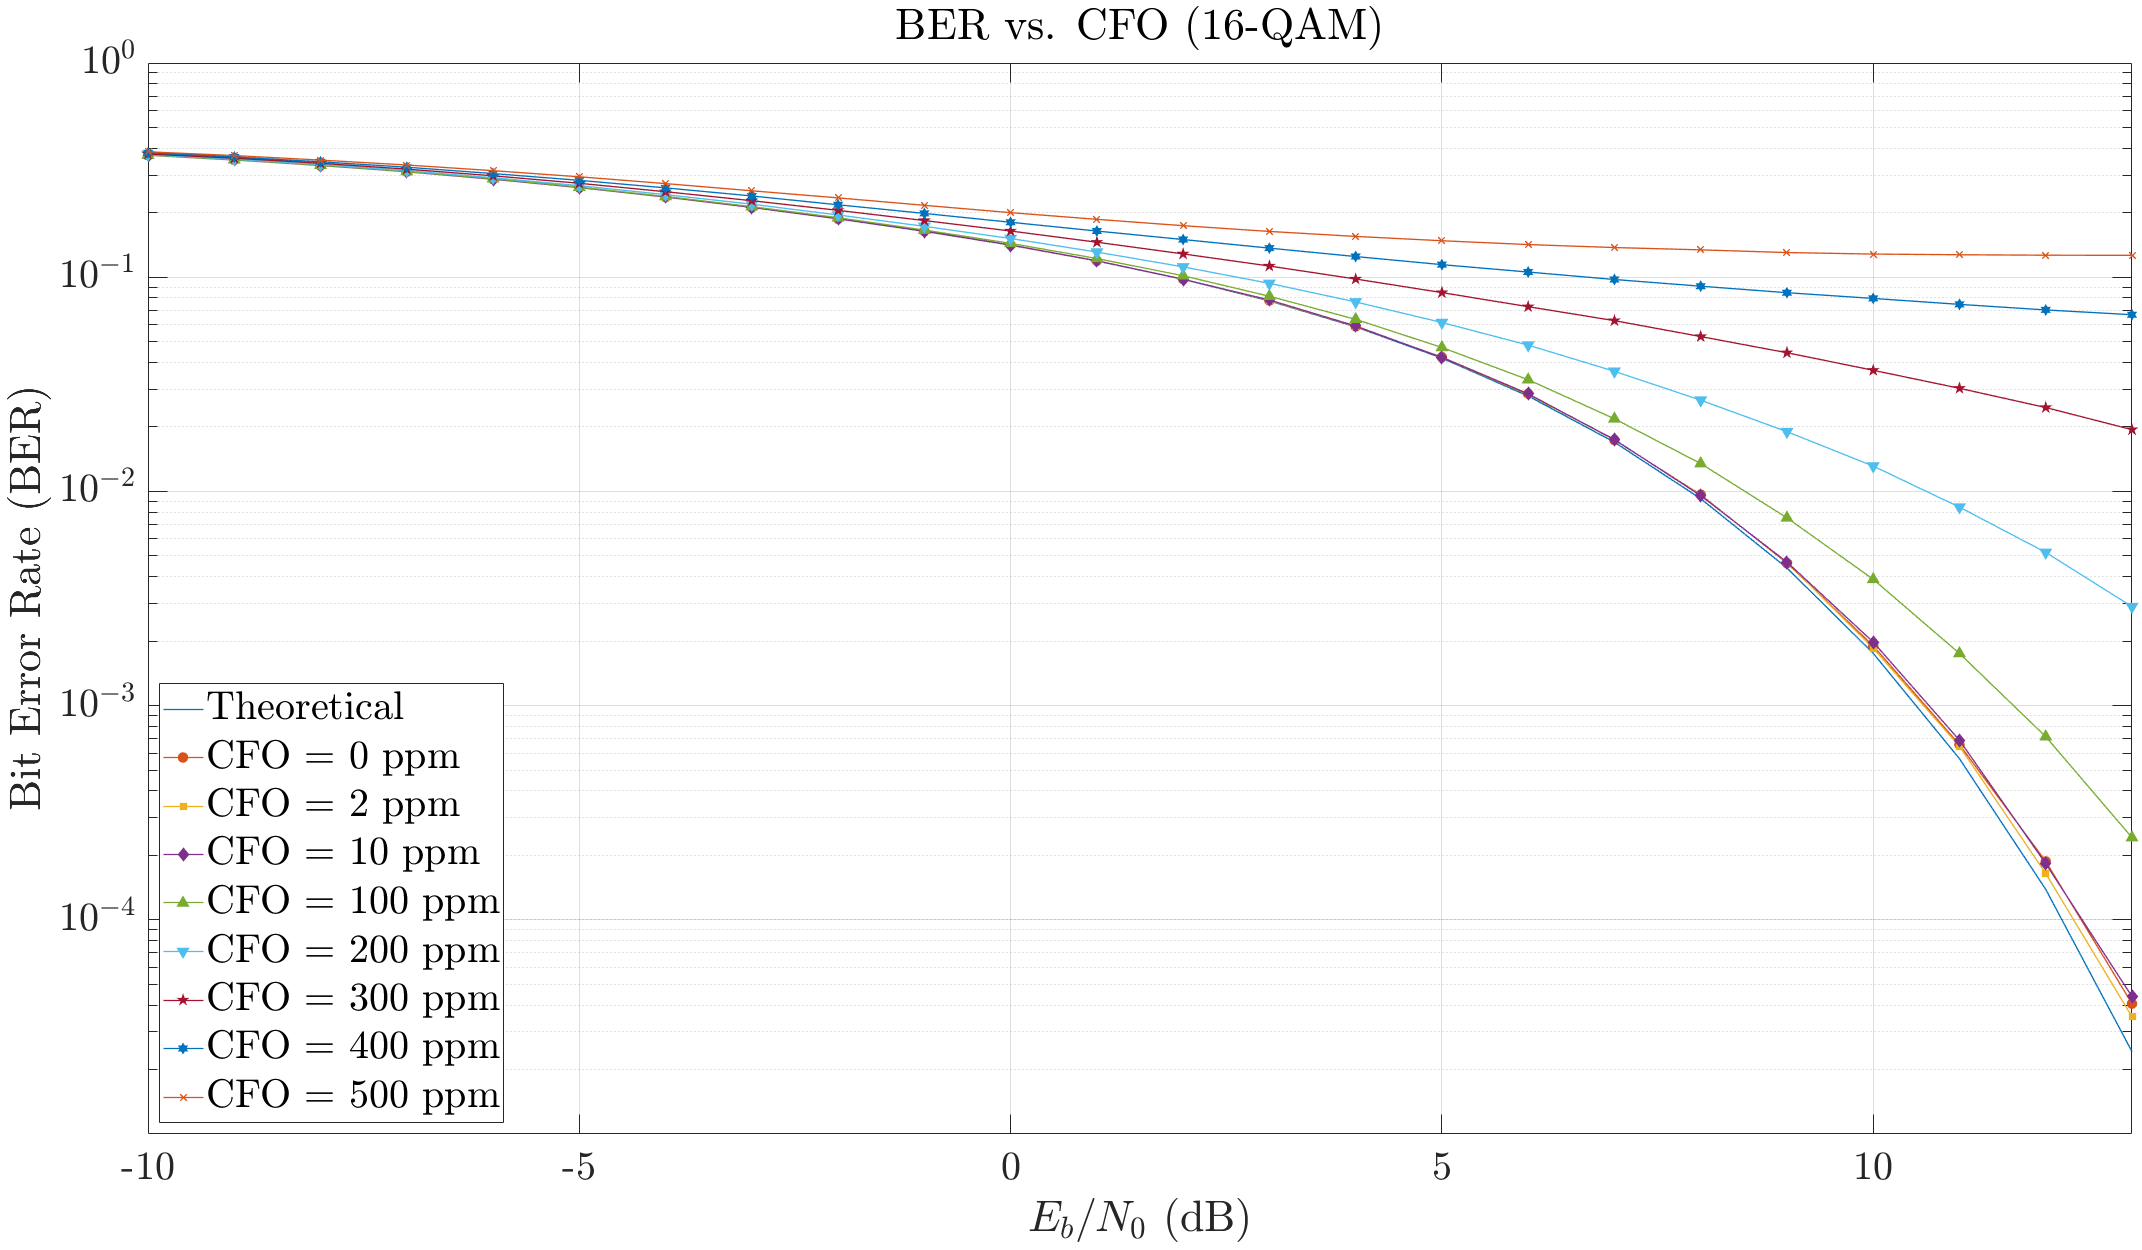
\includegraphics[width=\linewidth]{ber-cfo}
    \caption{Simulated BER vs. $E_b/N_0$ for 16-QAM with varying CFO}
    \label{fig:ber-cfo}
\end{figure}
A carrier frequency offset $\Delta f$ means that the received signal before matched filtering can be modeled as $r(t) = s(t) e^{j(2\pi \Delta f t)}$, (assuming no phase offset and no noise). The impacts of CFO are:
\begin{enumerate}
    \item Phase Drift: After matched filtering and sampling at $t = nT_{symb}$, each symbol $I[n]$ experiences a progressively changing phase rotation: $y[n] = I[n] e^{j(2\pi \Delta f nT_{symb})}$. This causes the received constellation points to form circles if uncorrected. Figure \ref{fig:cfo-po-sub} illustrates this for a 16-QAM constellation at an $E_b/N_0$ of 15 dB; the received symbols are smeared along arcs around the ideal transmitted symbol locations due to this progressive phase change and an initial phase offset.
    \item Inter-Symbol Interference: If the CFO is significant, the received signal's spectrum is shifted. Consequently, the receiver's filter $g^*(-t)$ is no longer perfectly matched to the incoming signal component $g(t)e^{j2\pi \Delta f t}$, leading to a loss in SNR and the introduction of ISI. The overall degradation in Bit Error Rate due to CFO is quantified in Figure \ref{fig:ber-cfo} for a 16-QAM system. A CFO of 100 ppm, for instance, requires approximately 2 dB more $E_b/N_0$ to achieve a BER of $10^{-3}$ compared to the theoretical curve. As CFO increases, performance deteriorates further, exhibiting even more errors due to the combined impact of ISI and phase drift.
\end{enumerate}

\subsubsection{Impact of Sample Time Shift ($t_0$)}
\begin{figure}[H]
    \centering
    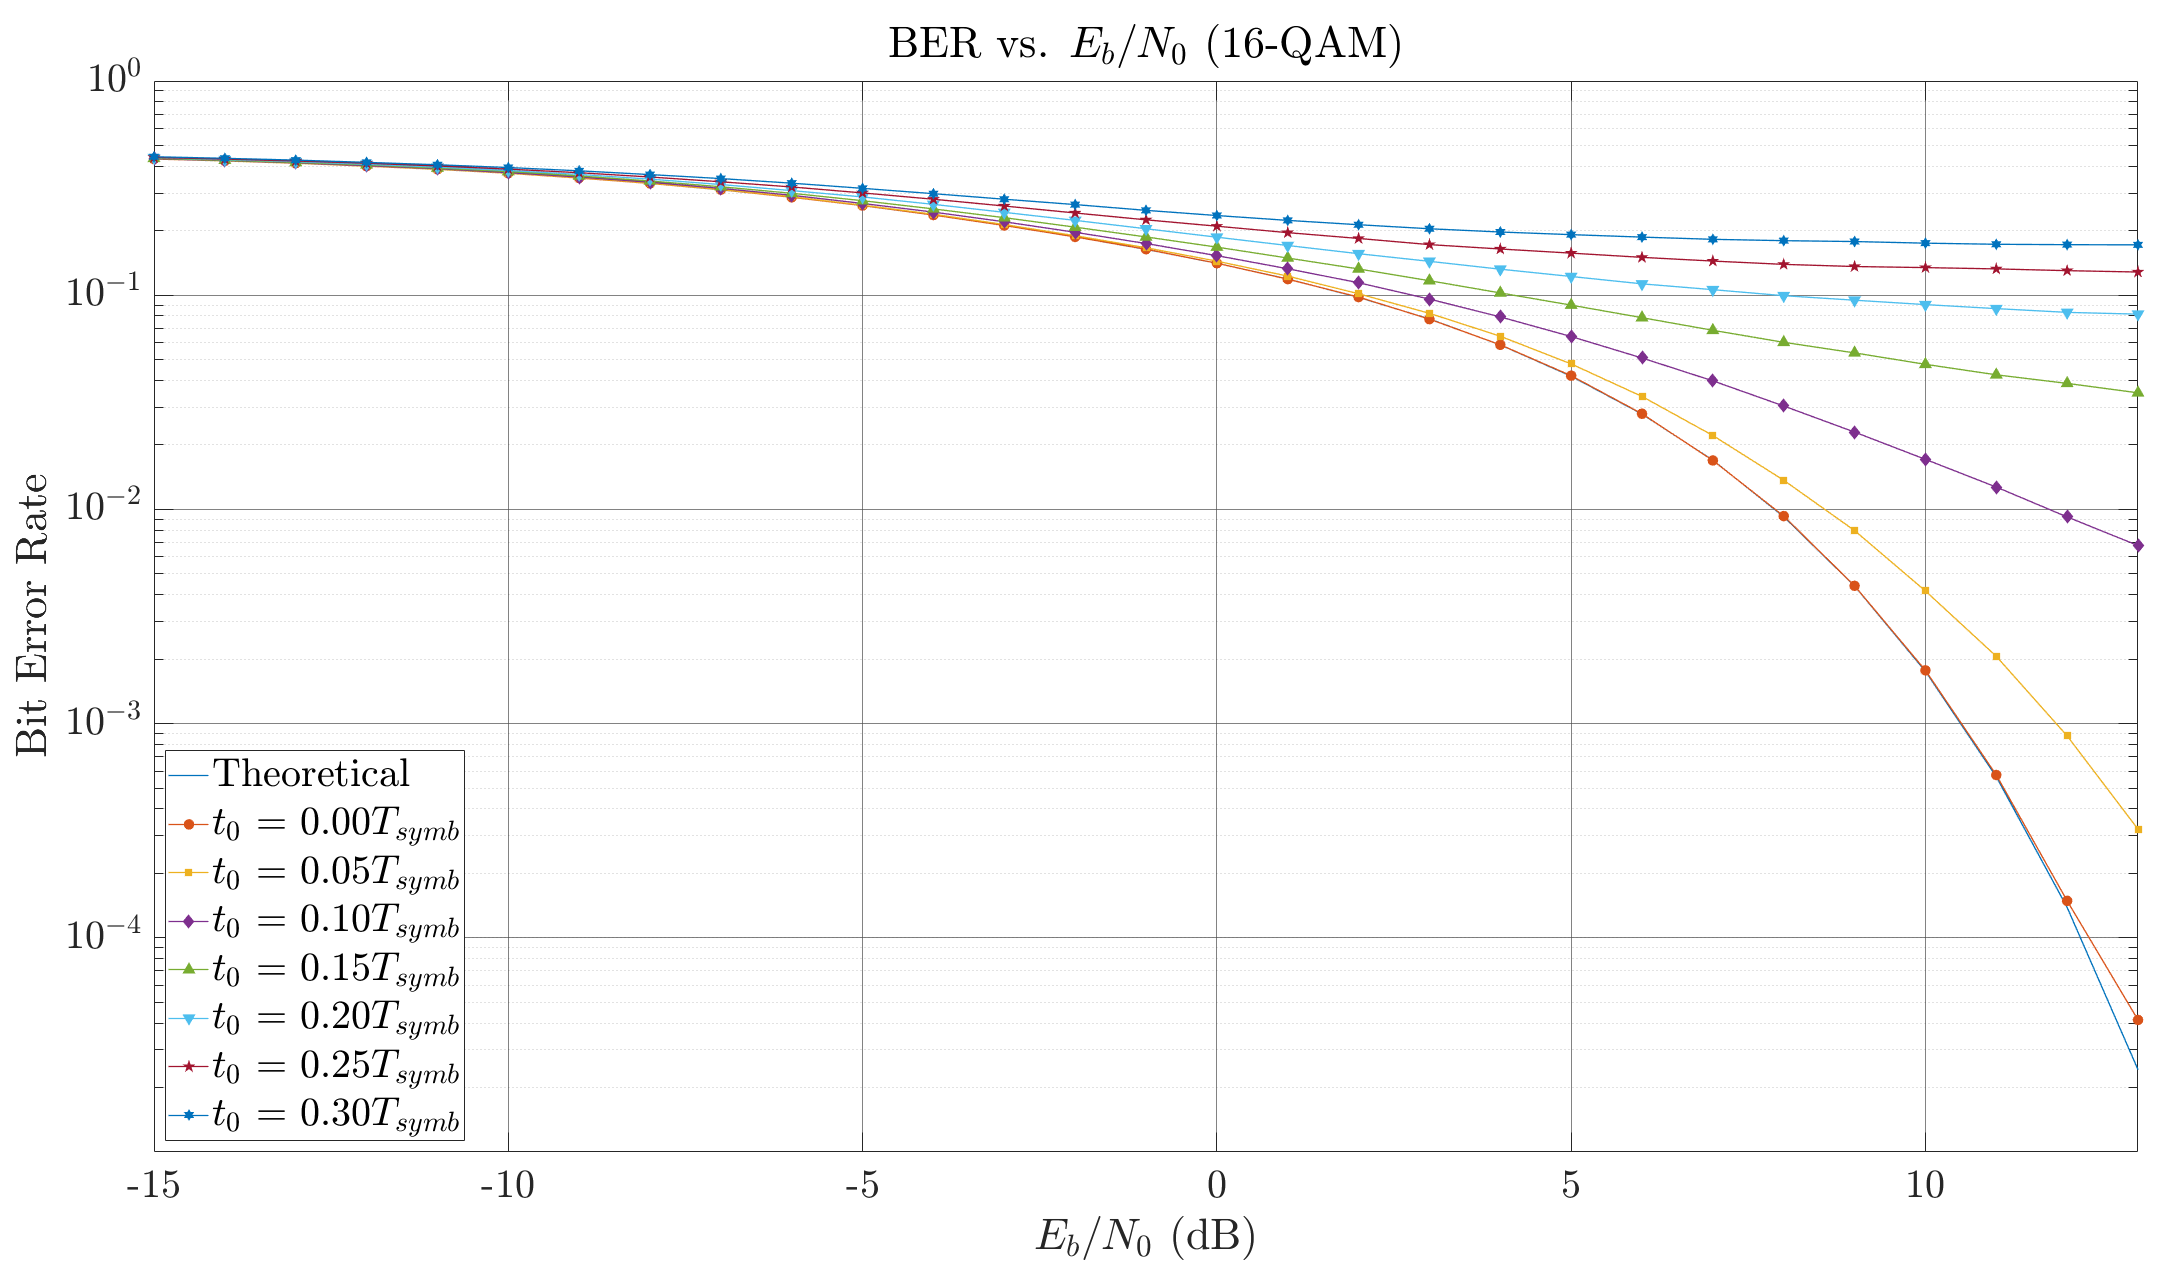
\includegraphics[width=\linewidth]{ber-timing}
    \caption{Simulated BER vs. $E_b/N_0$ for 16-QAM with varying timing offsets}
    \label{fig:ber-timing}
\end{figure}
An incorrect sampling instant $t_0 \neq 0$, relative to the optimal point means the matched filter output is not sampled at maximum signal energy and zero ISI. If $h(t)$ is the overall Nyquist filter response, and assuming no noise, sampling at $nT_{symb} + t_0$ yields:
\begin{align}
	y[n] &= \sum_m I[m]h((n-m)T_{symb} + t_0) \\
	&= I[n]h(t_0) + \sum_{m \neq n} I[m]h((n-m)T_{symb} + t_0) \label{eq:timing_offset_impact_revised}
\end{align}

\par
The first term, $I[n]h(t_0)$, represents the attenuated desired symbol (since $h(t_0) < h(0)$ for $t_0 \neq 0$). The second term is the ISI, as $h(kT_{symb} + t_0)$ is non-zero for $k \neq 0$ when $t_0 \neq 0$. The performance degradation due to such timing offsets is illustrated in Figure \ref{fig:ber-timing} for a 16-QAM system. Increasing the timing offset from $t_0 = 0 T_{symb}$ to $0.3 T_{symb}$ results in a progressively worse BER.

\begin{figure}[H]
	\centering
	\begin{subfigure}[b]{0.48\textwidth}
		\centering
		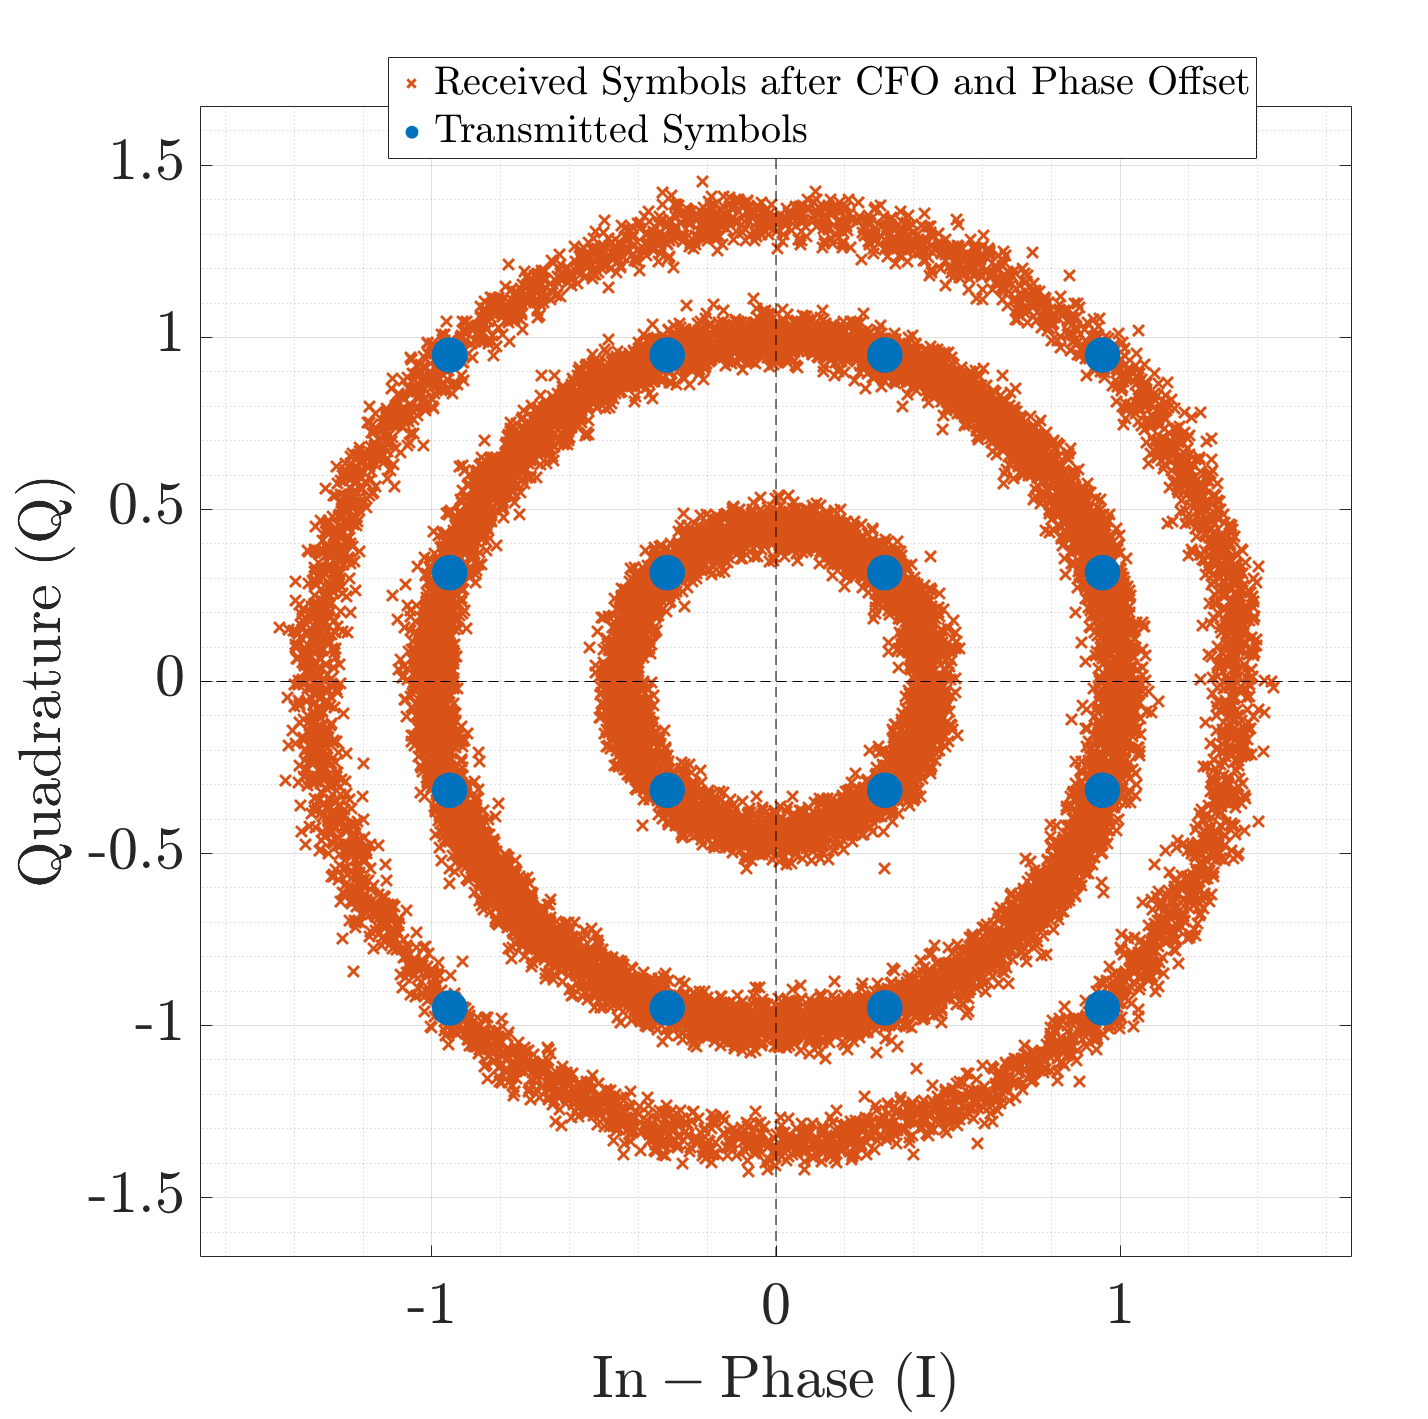
\includegraphics[width=\linewidth]{cfo-po}
		\caption{16-QAM Constellation diagram after CFO and Phase Offset}
		\label{fig:cfo-po-sub}
	\end{subfigure}
	\hfill 
	\begin{subfigure}[b]{0.48\textwidth}
		\centering
		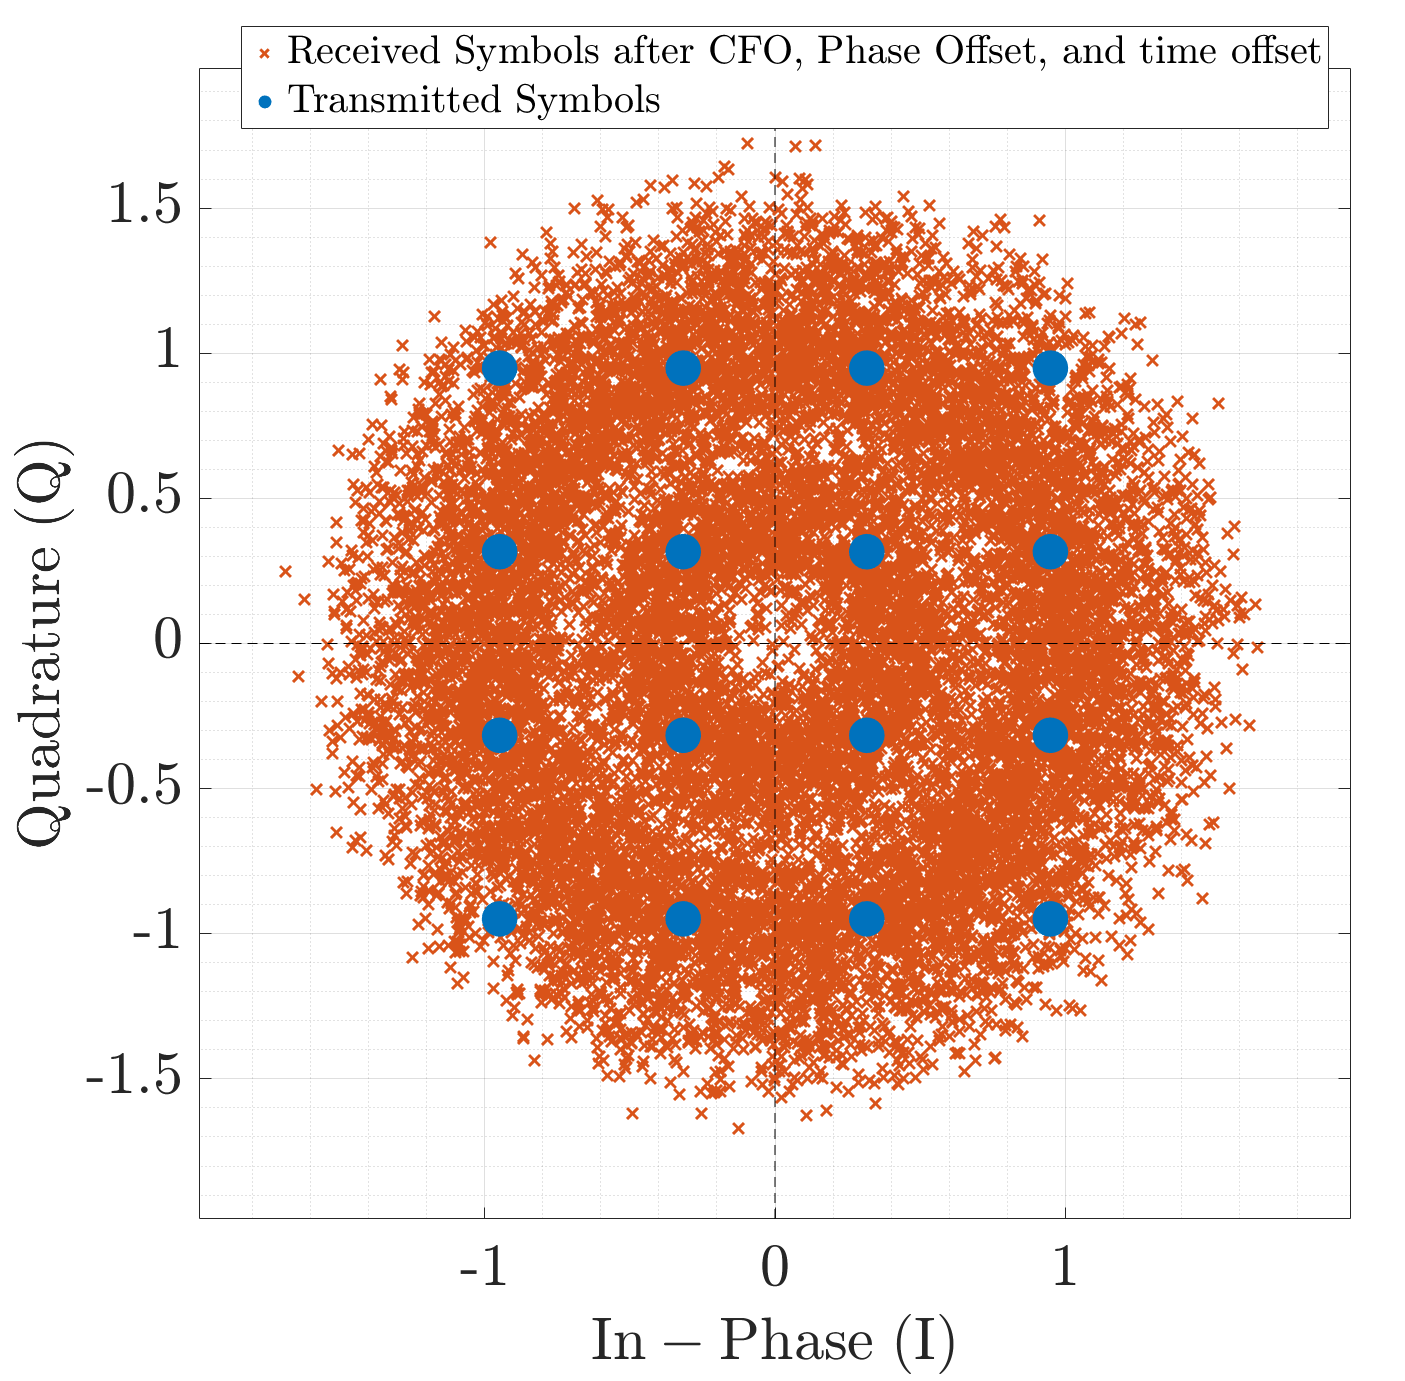
\includegraphics[width=\linewidth]{cfo-po-to}
		\caption{16-QAM Constellation diagram after CFO, Phase Offset and time offset}
		\label{fig:cfo-po-to-sub}
	\end{subfigure}
	\caption{Simulated Constellation diagrams of symbols transmitted and received after adding AWGN noise such that $\frac{E_b}{N_0} = 20$ dB, and filtering.}
	\label{fig:cfo-combined}
\end{figure}